
\newthought{The pages} of a book are usually divided into three major
sections: the front matter (also called preliminary matter or prelim), the
main matter (the core text of the book), and the back matter (or end
matter).

% \newthought{The front matter} of a book refers to all of the material that
% comes before the main text.  The following table from shows a list of
% material that appears in the front matter of \VDQI, \EI, \VE, and \BE
% along with its page number.  Page numbers that appear in parentheses refer
% to folios that do not have a printed page number (but they are still
% counted in the page number sequence).

% \bigskip
% \begin{minipage}{\textwidth}
% \begin{center}
% \begin{tabular}{lcccc}
% \toprule
%  & \multicolumn{4}{c}{Books} \\
% \cmidrule(l){2-5} 
% Page content & \vdqi & \ei & \ve & \be \\
% \midrule
% Blank half title page & \hangp{1} & \hangp{1} & \hangp{1} & \hangp{1} \\
% Frontispiece\footnotemark{}
%   & \hangp{2} & \hangp{2} & \hangp{2} & \hangp{2} \\
% Full title page & \hangp{3} & \hangp{3} & \hangp{3} & \hangp{3} \\
% Copyright page & \hangp{4} & \hangp{4} & \hangp{4} & \hangp{4} \\
% Contents & \hangp{5} & \hangp{5} & \hangp{5} & \hangp{5} \\
% %Blank & -- & \hangp{6} & \hangp{6} & \hangp{6} \\
% Dedication & \hangp{6} & \hangp{7} & \hangp{7} & 7 \\
% %Blank & -- & \hangp{8} & -- & \hangp{8} \\
% Epigraph & -- & -- & \hangp{8} & -- \\
% Introduction & \hangp{7} & \hangp{9} & \hangp{9} & 9 \\
% \bottomrule
% \end{tabular}
% \end{center}
% \end{minipage}
% \vspace{-7\baselineskip}\footnotetext{The contents of this page vary from book to book.  In
%   \vdqi this page is blank; in \ei and \ve this page holds a frontispiece;
%   and in \be this page contains three epigraphs.}
% \vspace{7\baselineskip}

\bigskip
The design of the front matter in Tufte's books varies slightly from the
traditional design of front matter.  First, the pages in front matter are
traditionally numbered with lowercase roman numerals (\eg, i, ii, iii,
iv,~\ldots).  Second, the front matter page numbering sequence is usually
separate from the main matter page numbering.  That is, the page numbers
restart at 1 when the main matter begins.  In contrast, Tufte has
enumerated his pages with arabic numerals that share the same page counting
sequence as the main matter.  

% There are also some variations in design across Tufte's four books.  The
% page opposite the full title page (labeled ``frontispiece'' in the above
% table) has different content in each of the books.  In \VDQI, this page is
% blank; in \EI and \VE, this page holds a frontispiece; and in \BE, this
% page contains three epigraphs.

% The dedication appears on page~6 in \vdqi (opposite the introduction), and
% is placed on its own spread in the other books.  In \ve, an epigraph shares
% the spread with the opening page of the introduction.

% None of the page numbers (folios) of the front matter are expressed except in
% \be, where the folios start to appear on the dedication page.

\newthought{The full title page} of each of the books varies slightly in
design.  In all the books, the author's name appears at the top of the
page, the title it set just above the center line, and the publisher is
printed along the bottom margin.  Some of the differences are outlined in
the following table.

% \bigskip
% \begin{center}
% \footnotesize
% \begin{tabular}{lllll}
% \toprule
% Feature & \vdqi & \ei & \ve & \be \\
% \midrule
% Author & & & & \\
% \quad Typeface & serif   & serif   & serif   & sans serif \\
% \quad Style    & italics & italics & italics & upright, caps \\
% \quad Size     & 24 pt   & 20 pt   & 20 pt   & 20 pt \\
% \addlinespace
% Title & & & & \\
% \quad Typeface & serif   & serif   & serif   & sans serif \\
% \quad Style    & upright & italics & upright & upright, caps \\
% \quad Size     & 36 pt   & 48 pt   & 48 pt   & 36 pt \\
% \addlinespace
% Subtitle & & & & \\
% \quad Typeface & \na     & \na     & serif   & \na \\
% \quad Style    & \na     & \na     & upright & \na \\
% \quad Size     & \na     & \na     & 20 pt   & \na \\
% \addlinespace
% Edition & & & & \\
% \quad Typeface & sans serif    & \na  & \na  & \na \\
% \quad Style    & upright, caps & \na  & \na  & \na \\
% \quad Size     & 14 pt         & \na  & \na  & \na \\
% \addlinespace
% Publisher & & & & \\
% \quad Typeface & serif   & serif   & serif   & sans serif \\
% \quad Style    & italics & italics & italics & upright, caps \\
% \quad Size     & 14 pt   & 14 pt   & 14 pt   & 14 pt \\
% \bottomrule
% \end{tabular}
% \end{center}

% \begin{figure*}[p]
% \fbox{\includegraphics[width=0.45\linewidth]{vdqi-title.pdf}}
% \hfill
% \fbox{\includegraphics[width=0.45\linewidth]{ei-title.pdf}}
% \\\vspace{\baselineskip}
% \fbox{\includegraphics[width=0.45\linewidth]{ve-title.pdf}}
% \hfill
% \fbox{\includegraphics[width=0.45\linewidth]{be-title.pdf}}
% \end{figure*}

% \newthought{The tables of contents} in Tufte's books give us our first
% glimpse of the structure of the main matter.  \VDQI is split into two
% parts, each containing some number of chapters.  His other three books only
% contain chapters---they're not broken into parts.

% \begin{figure*}[p]\index{table of contents}
% \fbox{\includegraphics[width=0.45\linewidth]{vdqi-contents.pdf}}
% \hfill
% \fbox{\includegraphics[width=0.45\linewidth]{ei-contents.pdf}}
% \\\vspace{\baselineskip}
% \fbox{\includegraphics[width=0.45\linewidth]{ve-contents.pdf}}
% \hfill
% \fbox{\includegraphics[width=0.45\linewidth]{be-contents.pdf}}
% \end{figure*}


\section{Typefaces}\label{sec:typefaces1}\index{typefaces}
\index{fonts|see{typefaces}}

% Tufte's books primarily use two typefaces: Bembo and Gill Sans.  Bembo is used
% for the headings and body text, while Gill Sans is used for the title page and
% opening epigraphs in \BE.

% Since neither Bembo nor Gill Sans are available in default \LaTeX{}
% installations, the \TL document classes default to using Palatino and
% Helvetica, respectively.  In addition, the Bera Mono typeface is used for
% \texttt{monospaced} type.

% The following font sizes are defined by the \TL classes:

% \begin{table}[h]\index{typefaces!sizes}
%   \footnotesize%
%   \begin{center}
%     \begin{tabular}{lccl}
%       \toprule
%       \LaTeX{} size & Font size & Leading & Used for \\
%       \midrule
%       \verb+\tiny+         &  5 &  6 & sidenote numbers \\
%       \verb+\scriptsize+   &  7 &  8 & \na \\
%       \verb+\footnotesize+ &  8 & 10 & sidenotes, captions \\
%       \verb+\small+        &  9 & 12 & quote, quotation, and verse environments \\
%       \verb+\normalsize+   & 10 & 14 & body text \\
%       \verb+\large+        & 11 & 15 & \textsc{b}-heads \\
%       \verb+\Large+        & 12 & 16 & \textsc{a}-heads, \textsc{toc} entries, author, date \\
%       \verb+\LARGE+        & 14 & 18 & handout title \\
%       \verb+\huge+         & 20 & 30 & chapter heads \\
%       \verb+\Huge+         & 24 & 36 & part titles \\
%       \bottomrule
%     \end{tabular}
%   \end{center}
%   \caption{A list of \LaTeX{} font sizes as defined by the \TL document classes.}
%   \label{tab:font-sizes}
% \end{table}

\section{Headings}\label{sec:headings1}\index{headings}

Tufte's books include the following heading levels: parts,
chapters,\sidenote{Parts and chapters are defined for the \texttt{tufte-book}
class only.}  sections, subsections, and paragraphs.  Not defined by default
are: sub-subsections and subparagraphs.

% \begin{table}[h]
%   \begin{center}
%     \footnotesize%
%     \begin{tabular}{lcr}
%       \toprule
%       Heading & Style & Size \\
%       \midrule
%       Part & roman & \measure{24}{36}{40} \\
%       Chapter & italic & \measure{20}{30}{40} \\
%       Section & italic & \measure{12}{16}{26} \\
%       Subsection & italic & \measure{11}{15}{26} \\
%       Paragraph & italic & 10/14 \\
%       \bottomrule
%     \end{tabular}
%   \end{center}
%   \caption{Heading styles used in \BE.}
%   \label{tab:heading-styles}
% \end{table}

\paragraph{Paragraph} Paragraph headings (as shown here) are introduced by
italicized text and separated from the main paragraph by a bit of space.

\section{Environments}

The following characteristics define the various environments:


% \begin{table}[h]
%   \begin{center}
%     \footnotesize%
%     \begin{tabular}{lcl}
%       \toprule
%       Environment & Font size & Notes \\
%       \midrule
%       Body text & \measure{10}{14}{26} & \\
%       Block quote & \measure{9}{12}{24} & Block indent (left and right) by \unit[1]{pc} \\
%       Sidenotes & \measure{8}{10}{12} & Sidenote number is set inline, followed by word space \\
%       Captions & \measure{8}{10}{12} &  \\
%       \bottomrule
%     \end{tabular}
%   \end{center}
%   \caption{Environment styles used in \BE.}
%   \label{tab:environment-styles}
% \end{table}


\chapter[On the Use of the tufte-book Document Class]{On the Use of the \texttt{tufte-book} Document Class}
\label{ch:tufte-book}

The \TL document classes define a style similar to the
style Edward Tufte uses in his books and handouts.  Tufte's style is known
for its extensive use of sidenotes, tight integration of graphics with
text, and well-set typography.  This document aims to be at once a
demonstration of the features of the \TL document classes
and a style guide to their use.

\section{Page Layout}\label{sec:page-layout}
\subsection{Headings}\label{sec:headings}\index{headings}
This style provides \textsc{a}- and \textsc{b}-heads (that is,
\Verb|\section| and \Verb|\subsection|), demonstrated above.

If you need more than two levels of section headings, you'll have to define
them yourself at the moment; there are no pre-defined styles for anything below
a \Verb|\subsection|.  As Bringhurst points out in \textit{The Elements of
Typographic Style},\cite{Bringhurst2005} you should ``use as many levels of
headings as you need: no more, and no fewer.''

% The \TL classes will emit an error if you try to use
% \linebreak\Verb|\subsubsection| and smaller headings.

% let's start a new thought -- a new section
\newthought{In his later books},\cite{Tufte2006} Tufte
starts each section with a bit of vertical space, a non-indented paragraph,
and sets the first few words of the sentence in \textsc{small caps}.  To
accomplish this using this style, use the \doccmddef{newthought} command:
\begin{docspec}
  \doccmd{newthought}\{In his later books\}, Tufte starts\ldots
\end{docspec}


\section{Sidenotes}\label{sec:sidenotes}
One of the most prominent and distinctive features of this style is the
extensive use of sidenotes.  There is a wide margin to provide ample room
for sidenotes and small figures.  Any \doccmd{footnote}s will automatically
be converted to sidenotes.\footnote{This is a sidenote that was entered
using the \texttt{\textbackslash footnote} command.}  If you'd like to place ancillary
information in the margin without the sidenote mark (the superscript
number), you can use the \doccmd{marginnote} command.\marginnote{This is a
margin note.  Notice that there isn't a number preceding the note, and
there is no number in the main text where this note was written.}

The specification of the \doccmddef{sidenote} command is:
\begin{docspec}
  \doccmd{sidenote}[\docopt{number}][\docopt{offset}]\{\docarg{Sidenote text.}\}
\end{docspec}

Both the \docopt{number} and \docopt{offset} arguments are optional.  If you
provide a \docopt{number} argument, then that number will be used as the
sidenote number.  It will change of the number of the current sidenote only and
will not affect the numbering sequence of subsequent sidenotes.

Sometimes a sidenote may run over the top of other text or graphics in the
margin space.  If this happens, you can adjust the vertical position of the
sidenote by providing a dimension in the \docopt{offset} argument.  Some
examples of valid dimensions are:
\begin{docspec}
  \ttfamily 1.0in \qquad 2.54cm \qquad 254mm \qquad 6\Verb|\baselineskip|
\end{docspec}
If the dimension is positive it will push the sidenote down the page; if the
dimension is negative, it will move the sidenote up the page.

While both the \docopt{number} and \docopt{offset} arguments are optional, they
must be provided in order.  To adjust the vertical position of the sidenote
while leaving the sidenote number alone, use the following syntax:
\begin{docspec}
  \doccmd{sidenote}[][\docopt{offset}]\{\docarg{Sidenote text.}\}
\end{docspec}
The empty brackets tell the \Verb|\sidenote| command to use the default
sidenote number.

If you \emph{only} want to change the sidenote number, however, you may
completely omit the \docopt{offset} argument:
\begin{docspec}
  \doccmd{sidenote}[\docopt{number}]\{\docarg{Sidenote text.}\}
\end{docspec}

The \doccmddef{marginnote} command has a similar \docarg{offset} argument:
\begin{docspec}
  \doccmd{marginnote}[\docopt{offset}]\{\docarg{Margin note text.}\}
\end{docspec}

\section{References}
References are placed alongside their citations as sidenotes,
as well.  This can be accomplished using the normal \doccmddef{cite}
command.\sidenote{The first paragraph of this document includes a citation.}

The complete list of references may also be printed automatically by using
the \doccmddef{bibliography} command.  (See the end of this document for an
example.)  If you do not want to print a bibliography at the end of your
document, use the \doccmddef{nobibliography} command in its place.  

To enter multiple citations at one location,\cite[-3\baselineskip]{Tufte2006,Tufte1990} you can
provide a list of keys separated by commas and the same optional vertical
offset argument: \Verb|\cite{Tufte2006,Tufte1990}|.  
\begin{docspec}
  \doccmd{cite}[\docopt{offset}]\{\docarg{bibkey1,bibkey2,\ldots}\}
\end{docspec}

\section{Figures and Tables}\label{sec:figures-and-tables}
Images and graphics play an integral role in Tufte's work.
In addition to the standard \docenvdef{figure} and \docenvdef{tabular} environments,
this style provides special figure and table environments for full-width
floats.

Full page--width figures and tables may be placed in \docenvdef{figure*} or
\docenvdef{table*} environments.  To place figures or tables in the margin,
use the \docenvdef{marginfigure} or \docenvdef{margintable} environments as follows
(see figure~\ref{fig:marginfig}):

\begin{marginfigure}%
  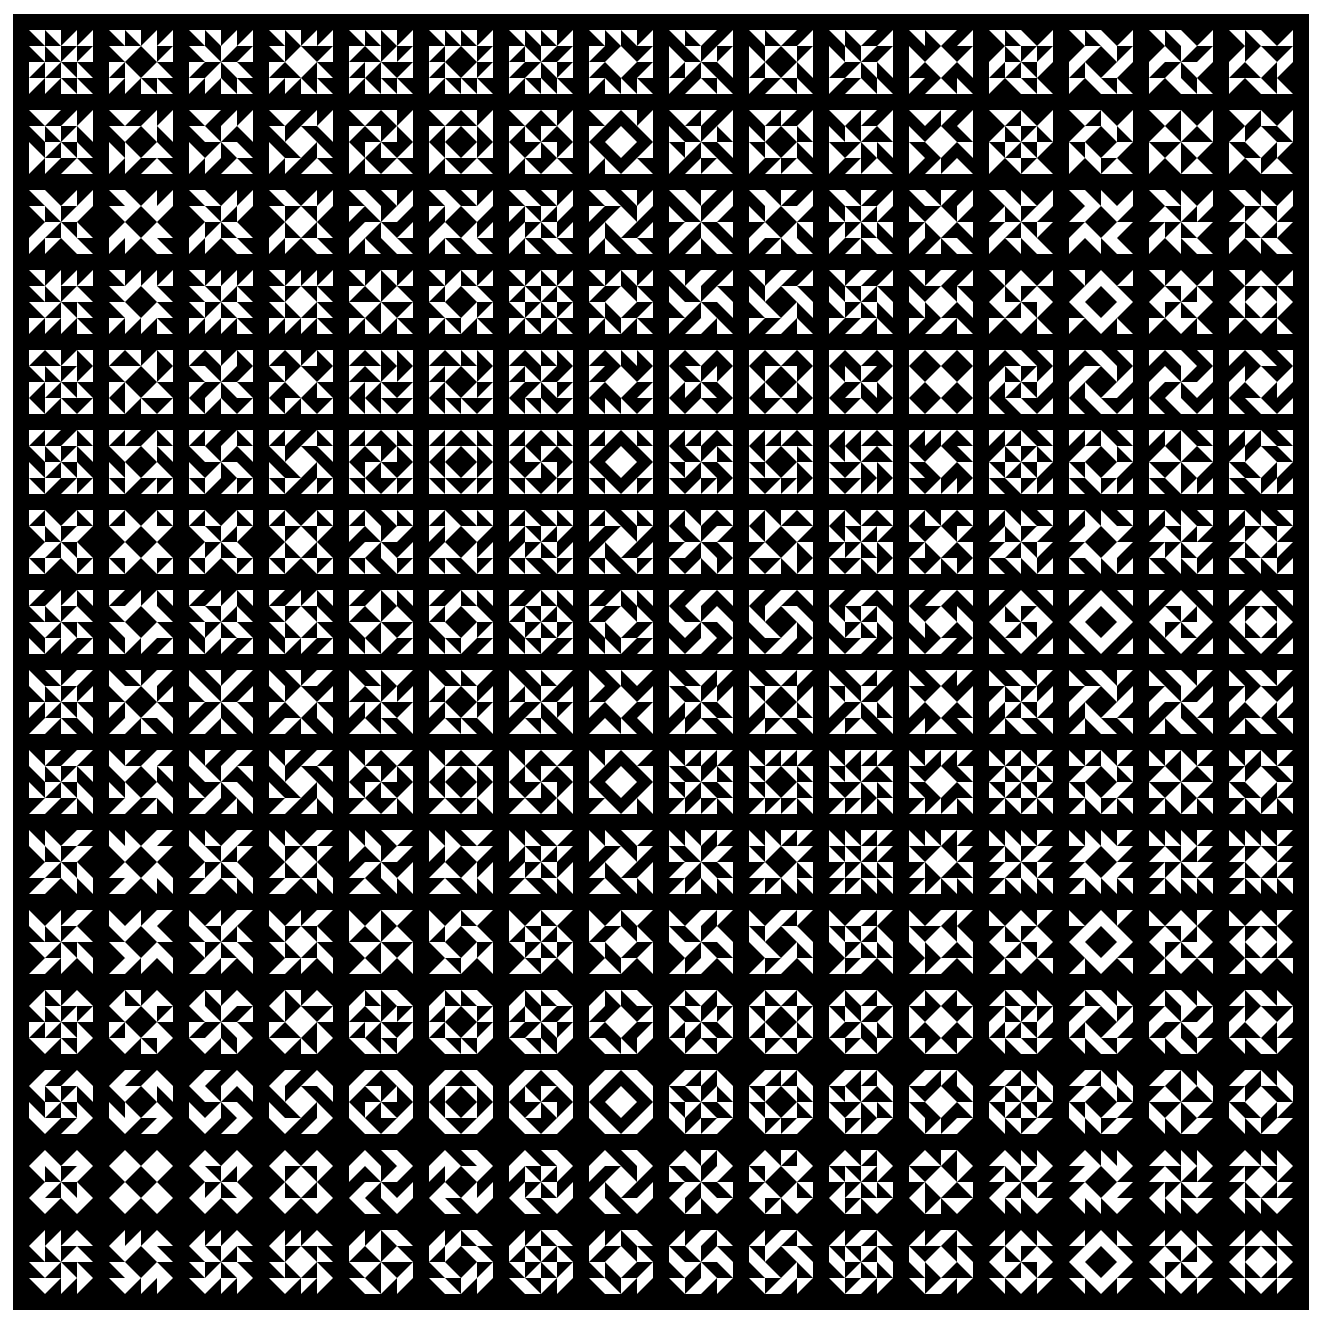
\includegraphics[width=\linewidth]{256.png}
  \caption{This is a margin figure.  The helix is defined by 
    $x = \cos(2\pi z)$, $y = \sin(2\pi z)$, and $z = [0, 2.7]$.  The figure was
    drawn using Asymptote (\url{http://asymptote.sf.net/}).}
  \label{fig:marginfig}
\end{marginfigure}

\begin{docspec}
\textbackslash begin\{marginfigure\}\\
  \qquad\textbackslash includegraphics\{256.png\}\\
  \qquad\textbackslash caption\{This is a margin figure.\}\\
  \qquad\textbackslash label\{fig:marginfig\}\\
\textbackslash end\{marginfigure\}\\
\end{docspec}

The \docenv{marginfigure} and \docenv{margintable} environments accept an optional parameter \docopt{offset} that adjusts the vertical position of the figure or table.  See the ``\nameref{sec:sidenotes}'' section above for examples.  The specifications are:
\begin{docspec}
  \textbackslash{begin\{marginfigure\}[\docopt{offset}]}\\
  \qquad\ldots\\
  \textbackslash{end\{marginfigure\}}\\
  \mbox{}\\
  \textbackslash{begin\{margintable\}[\docopt{offset}]}\\
  \qquad\ldots\\
  \textbackslash{end\{margintable\}}\\
\end{docspec}

Figure~\ref{fig:fullfig} is an example of the \docenv{figure*}
environment and figure~\ref{fig:textfig} is an example of the normal
\docenv{figure} environment.

\begin{figure*}[h]
  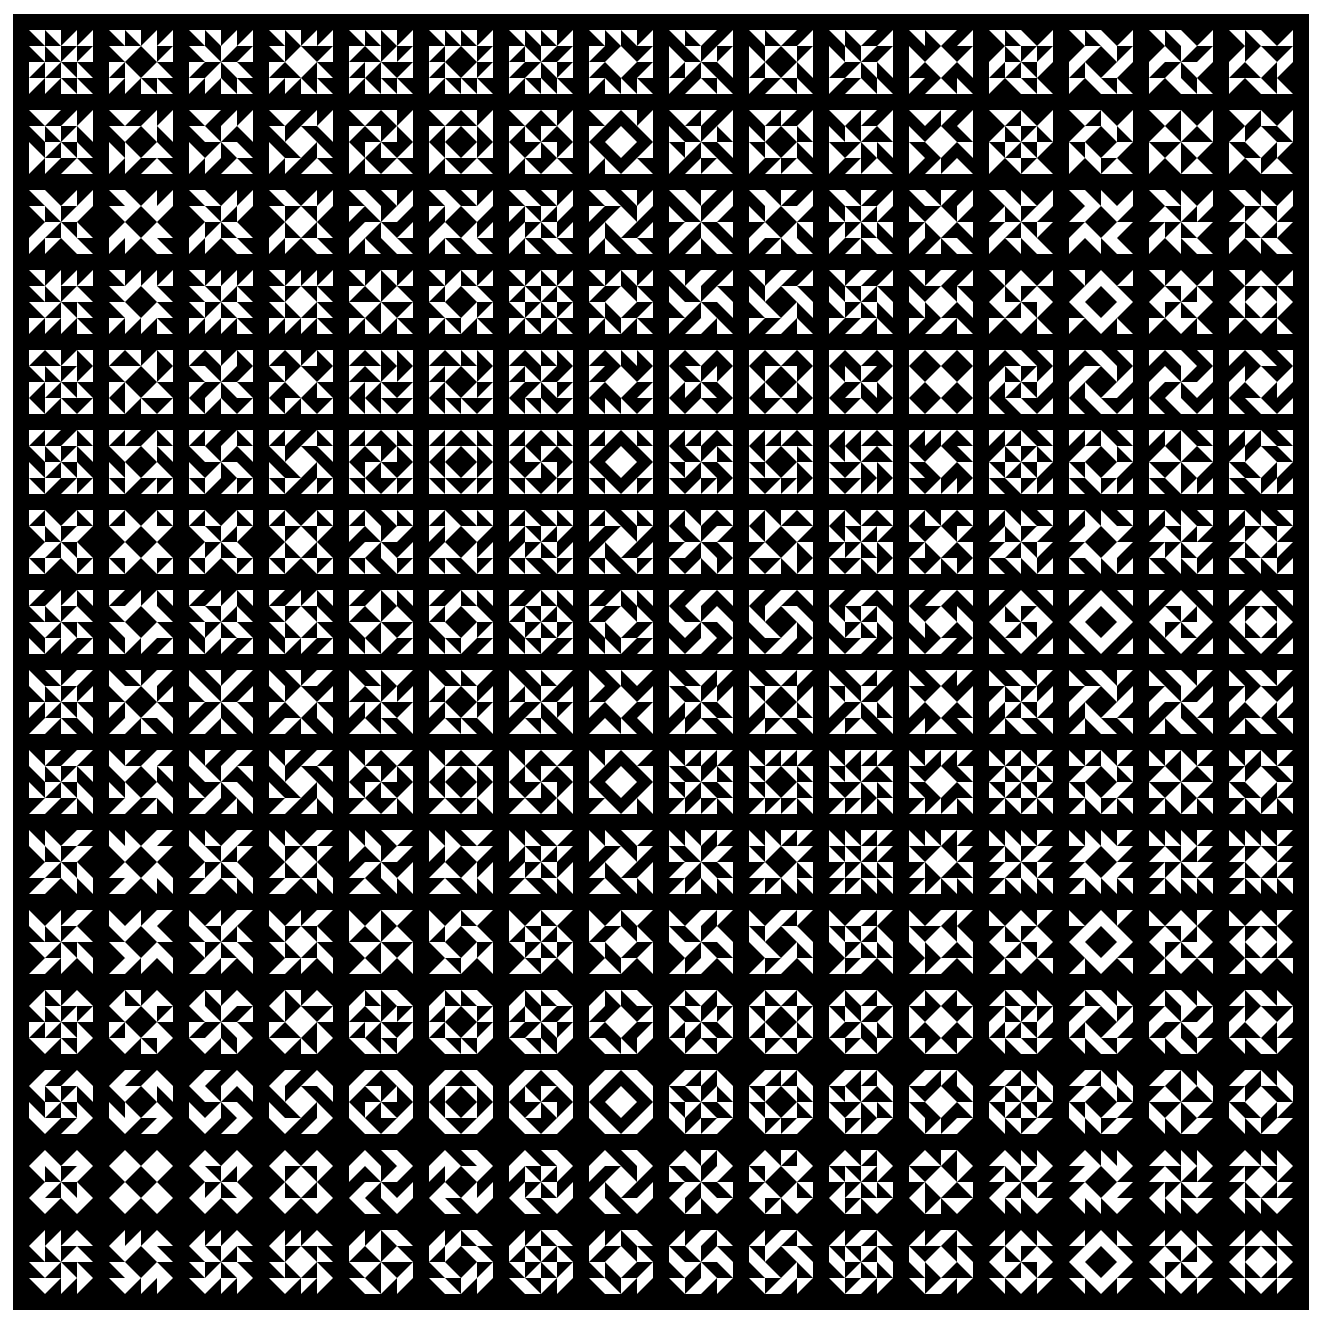
\includegraphics[width=\linewidth]{256.png}%
  \caption{This graph shows $y = \sin x$ from about $x = [-10, 10]$.
  \emph{Notice that this figure takes up the full page width.}}%
  \label{fig:fullfig}%
\end{figure*}

\begin{figure}
  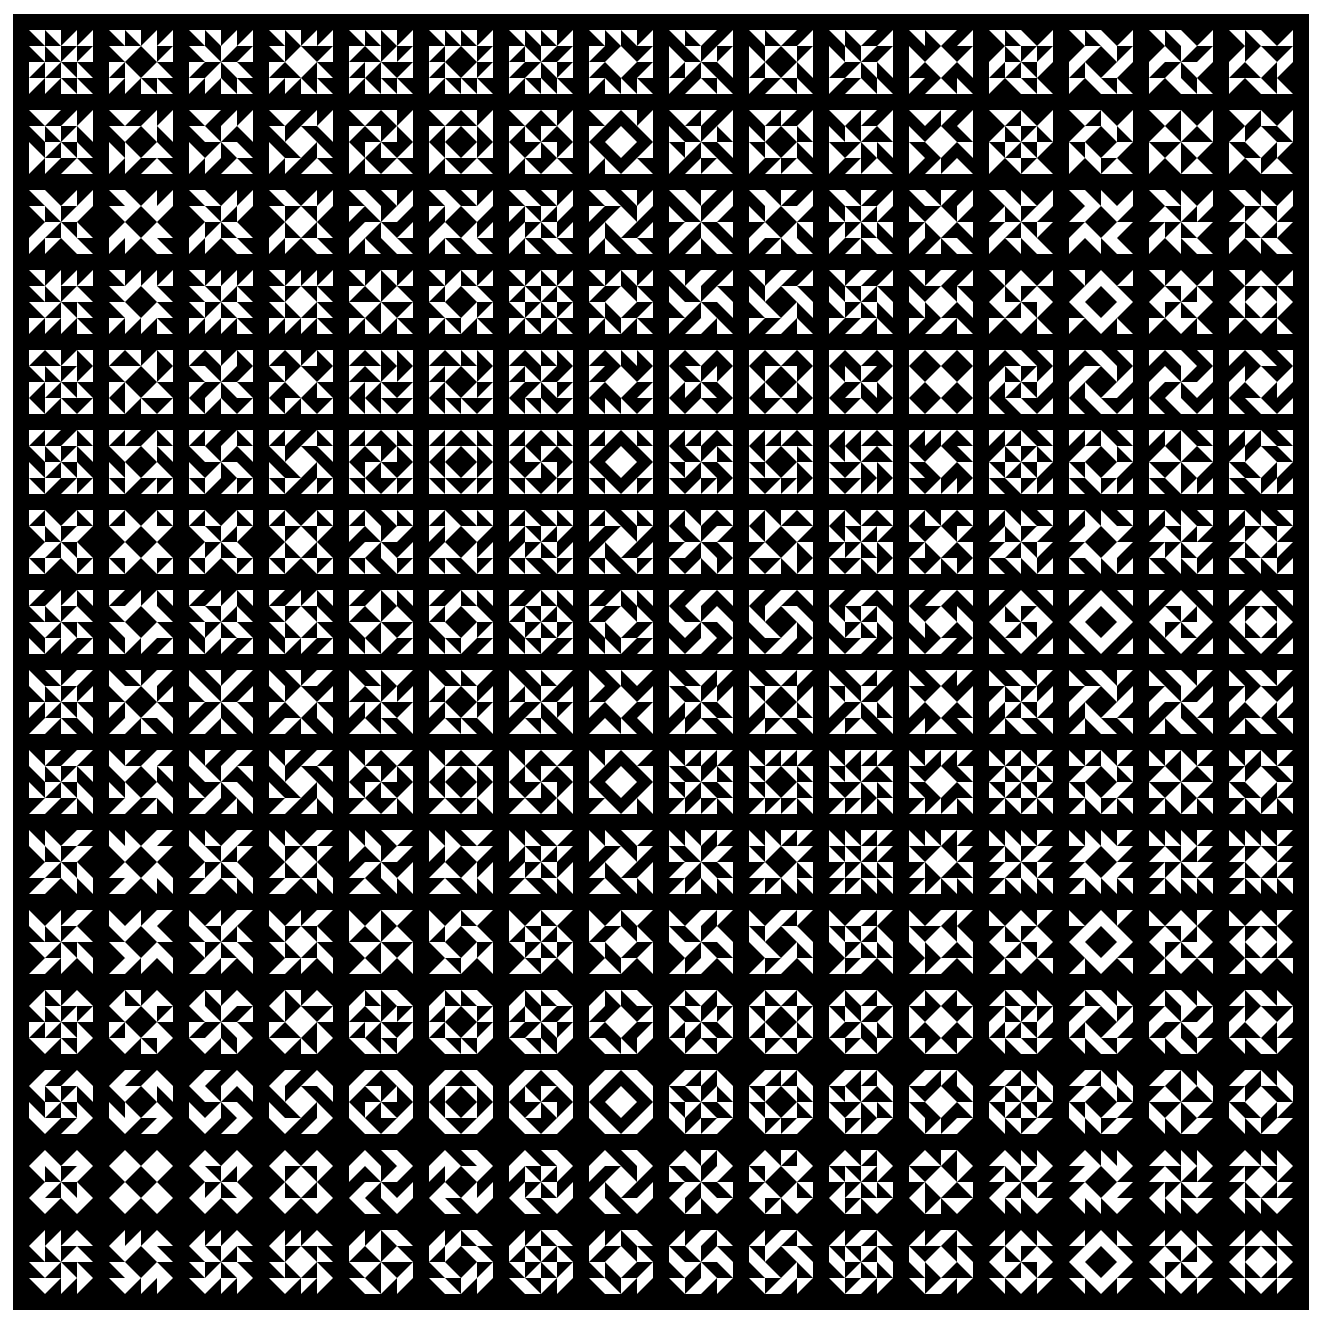
\includegraphics{256.png}
%  \checkparity This is an \pageparity\ page.%
  \caption[Hilbert curves of various degrees $n$.][6pt]{Hilbert curves of various degrees $n$. \emph{Notice that this figure only takes up the main textblock width.}}
  \label{fig:textfig}
  %\zsavepos{pos:textfig}
\end{figure}

As with sidenotes and marginnotes, a caption may sometimes require vertical
adjustment. The \doccmddef{caption} command now takes a second optional
argument that enables you to do this by providing a dimension \docopt{offset}.
You may specify the caption in any one of the following forms:
\begin{docspec}
  \doccmd{caption}\{\docarg{long caption}\}\\
  \doccmd{caption}[\docarg{short caption}]\{\docarg{long caption}\}\\
  \doccmd{caption}[][\docopt{offset}]\{\docarg{long caption}\}\\
  \doccmd{caption}[\docarg{short caption}][\docopt{offset}]%
                  \{\docarg{long caption}\}
\end{docspec}
A positive \docopt{offset} will push the caption down the page. The short
caption, if provided, is what appears in the list of figures/tables, otherwise
the ``long'' caption appears there. Note that although the arguments
\docopt{short caption} and \docopt{offset} are both optional, they must be
provided in order. Thus, to specify an \docopt{offset} without specifying a
\docopt{short caption}, you must include the first set of empty brackets
\Verb|[]|, which tell \doccmd{caption} to use the default ``long'' caption. As
an example, the caption to figure~\ref{fig:textfig} above was given in the form
\begin{docspec}
  \doccmd{caption}[Hilbert curves...][6pt]\{Hilbert curves...\}
\end{docspec}

Table~\ref{tab:normaltab} shows table created with the \docpkg{booktabs}
package.  Notice the lack of vertical rules---they serve only to clutter
the table's data.

\begin{table}[ht]
  \centering
  \fontfamily{ppl}\selectfont
  \begin{tabular}{ll}
    \toprule
    Margin & Length \\
    \midrule
    Paper width & \unit[8\nicefrac{1}{2}]{inches} \\
    Paper height & \unit[11]{inches} \\
    Textblock width & \unit[6\nicefrac{1}{2}]{inches} \\
    Textblock/sidenote gutter & \unit[\nicefrac{3}{8}]{inches} \\
    Sidenote width & \unit[2]{inches} \\
    \bottomrule
  \end{tabular}
  \caption{Here are the dimensions of the various margins used in the Tufte-handout class.}
  \label{tab:normaltab}
  %\zsavepos{pos:normaltab}
\end{table}

\newthought{Occasionally} \LaTeX{} will generate an error message:\label{err:too-many-floats}
\begin{docspec}
  Error: Too many unprocessed floats
\end{docspec}
\LaTeX{} tries to place floats in the best position on the page.  Until it's
finished composing the page, however, it won't know where those positions are.
If you have a lot of floats on a page (including sidenotes, margin notes,
figures, tables, etc.), \LaTeX{} may run out of ``slots'' to keep track of them
and will generate the above error.

% \LaTeX{} initially allocates 18 slots for storing floats.  To work around this
% limitation, the \TL document classes provide a \doccmddef{morefloats} command
% that will reserve more slots.

The first time \doccmd{morefloats} is called, it allocates an additional 34
slots.  The second time \doccmd{morefloats} is called, it allocates another 26
slots.

The \doccmd{morefloats} command may only be used two times.  Calling it a
third time will generate an error message.  (This is because we can't safely
allocate many more floats or \LaTeX{} will run out of memory.)

If, after using the \doccmd{morefloats} command twice, you continue to get the
\texttt{Too many unprocessed floats} error, there are a couple things you can
do.

The \doccmddef{FloatBarrier} command will immediately process all the floats
before typesetting more material.  Since \doccmd{FloatBarrier} will start a new
paragraph, you should place this command at the beginning or end of a
paragraph.

The \doccmddef{clearpage} command will also process the floats before
continuing, but instead of starting a new paragraph, it will start a new page.

You can also try moving your floats around a bit: move a figure or table to the
next page or reduce the number of sidenotes.  (Each sidenote actually uses
\emph{two} slots.)

After the floats have placed, \LaTeX{} will mark those slots as unused so they
are available for the next page to be composed.

% \section{Captions}
% You may notice that the captions are sometimes misaligned.
% Due to the way \LaTeX's float mechanism works, we can't know for sure where it
% decided to put a float. Therefore, the \TL document classes provide commands to
% override the caption position.

\paragraph{Vertical alignment} To override the vertical alignment, use the
\doccmd{setfloatalignment} command inside the float environment.  For
example:

\begin{fullwidth}
\begin{docspec}
  \textbackslash begin\{figure\}[btp]\\
  \qquad \textbackslash includegraphics\{256.png\}\\
  \qquad \textbackslash caption\{This is an example of a sine wave.\}\\
  \qquad \textbackslash label\{fig:sinewave\}\\
  \qquad \hlred{\textbackslash setfloatalignment\{b\}\% forces caption to be bottom-aligned}\\
  \textbackslash end\{figure\}
\end{docspec}
\end{fullwidth}

\noindent The syntax of the \doccmddef{setfloatalignment} command is:

\begin{docspec}
  \doccmd{setfloatalignment}\{\docopt{pos}\}
\end{docspec}

\noindent where \docopt{pos} can be either \texttt{b} for bottom-aligned
captions, or \texttt{t} for top-aligned captions.

\paragraph{Horizontal alignment}\label{par:overriding-horizontal}
To override the horizontal alignment, use either the \doccmd{forceversofloat}
or the \doccmd{forcerectofloat} command inside of the float environment.  For
example:

\begin{fullwidth}
\begin{docspec}
  \textbackslash begin\{figure\}[btp]\\
  \qquad \textbackslash includegraphics\{256.png\}\\
  \qquad \textbackslash caption\{This is an example of a sine wave.\}\\
  \qquad \textbackslash label\{fig:sinewave\}\\
  \qquad \hlred{\textbackslash forceversofloat\% forces caption to be set to the left of the float}\\
  \textbackslash end\{figure\}
\end{docspec}
\end{fullwidth}

The \doccmddef{forceversofloat} command causes the algorithm to assume the
float has been placed on a verso page---that is, a page on the left side of a
two-page spread.  Conversely, the \doccmddef{forcerectofloat} command causes
the algorithm to assume the float has been placed on a recto page---that is, a
page on the right side of a two-page spread.


\section{Full-width text blocks}

In addition to the new float types, there is a \docenvdef{fullwidth}
environment that stretches across the main text block and the sidenotes
area.

\begin{Verbatim}
\begin{fullwidth}
Lorem ipsum dolor sit amet...
\end{fullwidth}
\end{Verbatim}

\begin{fullwidth}
\small\itshape\lipsum[1]
\end{fullwidth}

\section{Typography}\label{sec:typography}

\subsection{Typefaces}\label{sec:typefaces}\index{typefaces}
If the Palatino, \textsf{Helvetica}, and \texttt{Bera Mono} typefaces are installed, this style
will use them automatically.  Otherwise, we'll fall back on the Computer Modern
typefaces.

\subsection{Letterspacing}\label{sec:letterspacing}
This document class includes two new commands and some improvements on
existing commands for letterspacing.

When setting strings of \allcaps{ALL CAPS} or \smallcaps{small caps}, the
letter\-spacing---that is, the spacing between the letters---should be
increased slightly.\cite{Bringhurst2005}  The \doccmddef{allcaps} command has proper letterspacing for
strings of \allcaps{FULL CAPITAL LETTERS}, and the \doccmddef{smallcaps} command
has letterspacing for \smallcaps{small capital letters}.  These commands
will also automatically convert the case of the text to upper- or
lowercase, respectively.

The \doccmddef{textsc} command has also been redefined to include
letterspacing.  The case of the \doccmd{textsc} argument is left as is,
however.  This allows one to use both uppercase and lowercase letters:
\textsc{The Initial Letters Of The Words In This Sentence Are Capitalized.}



\section{Document Class Options}\label{sec:options}

\index{class options|(}
The \doccls{tufte-book} class is based on the \LaTeX\ \doccls{book}
document class.  Therefore, you can pass any of the typical book
options.  There are a few options that are specific to the
\doccls{tufte-book} document class, however.

The \docclsoptdef{a4paper} option will set the paper size to \smallcaps{A4} instead of
the default \smallcaps{US} letter size.

The \docclsoptdef{sfsidenotes} option will set the sidenotes and title block in a 
\textsf{sans serif} typeface instead of the default roman.

The \docclsoptdef{twoside} option will modify the running heads so that the page
number is printed on the outside edge (as opposed to always printing the page
number on the right-side edge in \docclsoptdef{oneside} mode).  

The \docclsoptdef{symmetric} option typesets the sidenotes on the outside edge of
the page.  This is how books are traditionally printed, but is contrary to
Tufte's book design which sets the sidenotes on the right side of the page.
This option implicitly sets the \docclsopt{twoside} option.

The \docclsoptdef{justified} option sets all the text fully justified (flush left
and right).  The default is to set the text ragged right.  
The body text of Tufte's books are set ragged right.  This prevents
needless hyphenation and makes it easier to read the text in the slightly
narrower column.

The \docclsoptdef{bidi} option loads the \docpkg{bidi} package which is used with
\tXeLaTeX\ to typeset bi-directional text.  Since the \docpkg{bidi}
package needs to be loaded before the sidenotes and cite commands are defined,
it can't be loaded in the document preamble.

% The \docclsoptdef{debug} option causes the \TL classes to output debug
% information to the log file which is useful in troubleshooting bugs.  It will
% also cause the graphics to be replaced by outlines.

% The \docclsoptdef{nofonts} option prevents the \TL classes from
% automatically loading the Palatino and Helvetica typefaces.  You should use
% this option if you wish to load your own fonts.  If you're using \tXeLaTeX, this
% option is implied (\ie, the Palatino and Helvetica fonts aren't loaded if you
% use \tXeLaTeX).  

% The \docclsoptdef{nols} option inhibits the letterspacing code.  The \TL\
% classes try to load the appropriate letterspacing package (either pdf\TeX's
% \docpkg{letterspace} package or the \docpkg{soul} package).  If you're using
% \tXeLaTeX\ with \docpkg{fontenc}, however, you should configure your own
% letterspacing.  

% The \docclsoptdef{notitlepage} option causes \doccmd{maketitle} to generate a title
% block instead of a title page.  The \doccls{book} class defaults to a title
% page and the \doccls{handout} class defaults to the title block.  There is an
% analogous \docclsoptdef{titlepage} option that forces \doccmd{maketitle} to
% generate a full title page instead of the title block.

% The \docclsoptdef{notoc} option suppresses \TL's custom table of contents
% (\textsc{toc}) design.  The current \textsc{toc} design only shows unnumbered
% chapter titles; it doesn't show sections or subsections.  The \docclsopt{notoc}
% option will revert to \LaTeX's \textsc{toc} design.

The \docclsoptdef{nohyper} option prevents the \docpkg{hyperref} package from
being loaded.  The default is to load the \docpkg{hyperref} package and use the
\doccmd{title} and \doccmd{author} contents as metadata for the generated
\textsc{pdf}.

\index{class options|)}



\chapter[Customizing Tufte-LaTeX]{Customizing \TL}
\label{ch:customizing}

The \TL document classes are designed to closely emulate Tufte's book
design by default.  However, each document is different and you may encounter
situations where the default settings are insufficient.  This chapter explores
many of the ways you can adjust the \TL document classes to better fit
your needs.

\section{File Hooks}
\label{sec:filehooks}

\index{file hooks|(}
If you create many documents using the \TL classes, it's easier to
store your customizations in a separate file instead of copying them into the
preamble of each document.  The \TL classes provide three file hooks:
\docfilehook{tufte-common-local.tex}{common}, \docfilehook{tufte-book-local.tex}{book}, and
\docfilehook{tufte-handout-local.tex}{handout}.\sloppy

\begin{description}
  \item[\docfilehook{tufte-common-local.tex}{common}]
    If this file exists, it will be loaded by all of the \TL document
    classes just prior to any document-class-specific code.  If your
    customizations or code should be included in both the book and handout
    classes, use this file hook.
  \item[\docfilehook{tufte-book-local.tex}{book}] 
    If this file exists, it will be loaded after all of the common and
    book-specific code has been read.  If your customizations apply only to the
    book class, use this file hook.
  \item[\docfilehook{tufte-common-handout.tex}{handout}] 
    If this file exists, it will be loaded after all of the common and
    handout-specific code has been read.  If your customizations apply only to
    the handout class, use this file hook.
\end{description}

\index{file hooks|)}

\section{Numbered Section Headings}
\label{sec:numbered-sections}
\index{headings!numbered}

While Tufte dispenses with numbered headings in his books, if you require them,
they can be anabled by changing the value of the \doccounter{secnumdepth}
counter.  From the table below, select the heading level at which numbering
should stop and set the \doccounter{secnumdepth} counter to that value.  For
example, if you want parts and chapters numbered, but don't want numbering for
sections or subsections, use the command:
\begin{docspec}
  \doccmd{setcounter}\{secnumdepth\}\{0\}
\end{docspec}

The default \doccounter{secnumdepth} for the \TL document classes is $-1$.

\begin{table}
  \footnotesize
  \begin{center}
    \begin{tabular}{lr}
      \toprule
      Heading level & Value \\
      \midrule
      Part (in \doccls{tufte-book}) & $-1$ \\
      Part (in \doccls{tufte-handout}) & $0$ \\
      Chapter (only in \doccls{tufte-book}) & $0$ \\
      Section & $1$ \\
      Subsection & $2$ \\
      Subsubsection & $3$ \\
      Paragraph & $4$ \\
      Subparagraph & $5$ \\
      \bottomrule
    \end{tabular}
  \end{center}
  \caption{Heading levels used with the \texttt{secnumdepth} counter.}
\end{table}

\section{Changing the Paper Size}
\label{sec:paper-size}

The \TL classes currently only provide three paper sizes: \textsc{a4},
\textsc{b5}, and \textsc{us} letter.  To specify a different paper size (and/or
margins), use the \doccmd[geometry]{geometrysetup} command in the preamble of your
document (or one of the file hooks).  The full documentation of the
\doccmd{geometrysetup} command may be found in the \docpkg{geometry} package
documentation.\cite{pkg-geometry}


\section{Customizing Marginal Material}
\label{sec:marginal-material}

Marginal material includes sidenotes, citations, margin notes, and captions.
Normally, the justification of the marginal material follows the justification
of the body text.  If you specify the \docclsopt{justified} document class
option, all of the margin material will be fully justified as well.  If you
don't specify the \docclsopt{justified} option, then the marginal material will
be set ragged right.

You can set the justification of the marginal material separately from the body
text using the following document class options: \docclsopt{sidenote},
\docclsopt{marginnote}, \docclsopt{caption}, \docclsopt{citation}, and
\docclsopt{marginals}.  Each option refers to its obviously corresponding
marginal material type.  The \docclsopt{marginals} option simultaneously sets
the justification on all four marginal material types.

Each of the document class options takes one of five justification types:
\begin{description}
  \item[\docclsopt{justified}] Fully justifies the text (sets it flush left and
    right).
  \item[\docclsopt{raggedleft}] Sets the text ragged left, regardless of which
    page it falls on.
  \item[\docclsopt{raggedright}] Sets the text ragged right, regardless of
    which page it falls on.
  \item[\doccls{raggedouter}] Sets the text ragged left if it falls on the
    left-hand (verso) page of the spread and otherwise sets it ragged right.
    This is useful in conjunction with the \docclsopt{symmetric} document class
    option.
  \item[\docclsopt{auto}] If the \docclsopt{justified} document class option
    was specified, then set the text fully justified; otherwise the text is set
    ragged right.  This is the default justification option if one is not
    explicitly specified.
\end{description}

\noindent For example, 
\begin{docspec}
  \doccmdnoindex{documentclass}[symmetric,justified,marginals=raggedouter]\{tufte-book\}
\end{docspec}
will set the body text of the document to be fully justified and all of the
margin material (sidenotes, margin notes, captions, and citations) to be flush
against the body text with ragged outer edges.

\newthought{The font and style} of the marginal material may also be modified using the following commands:

\begin{docspec}
  \doccmd{setsidenotefont}\{\docopt{font commands}\}\\
  \doccmd{setcaptionfont}\{\docopt{font commands}\}\\
  \doccmd{setmarginnotefont}\{\docopt{font commands}\}\\
  \doccmd{setcitationfont}\{\docopt{font commands}\}
\end{docspec}

The \doccmddef{setsidenotefont} sets the font and style for sidenotes, the
\doccmddef{setcaptionfont} for captions, the \doccmddef{setmarginnotefont} for
margin notes, and the \doccmddef{setcitationfont} for citations.  The
\docopt{font commands} can contain font size changes (e.g.,
\doccmdnoindex{footnotesize}, \doccmdnoindex{Huge}, etc.), font style changes (e.g.,
\doccmdnoindex{sffamily}, \doccmdnoindex{ttfamily}, \doccmdnoindex{itshape}, etc.), color changes (e.g.,
\doccmdnoindex{color}\texttt{\{blue\}}), and many other adjustments.

If, for example, you wanted the captions to be set in italic sans serif, you could use:
\begin{docspec}
  \doccmd{setcaptionfont}\{\doccmdnoindex{itshape}\doccmdnoindex{sffamily}\}
\end{docspec}
